\documentclass[17pt]{beamer} %Makes presentation
%\documentclass[handout, 17pt]{beamer} %Makes Handouts
\documentclass[14pt]{beamer} %Makes presentation
%\documentclass[handout]{beamer} %Makes Handouts
\usetheme{Singapore} %Gray with fade at top
\useoutertheme[subsection=false]{miniframes} %Supppress subsection in header
\useinnertheme{rectangles} %Itemize/Enumerate boxes
\usecolortheme{seagull} %Color theme
\usecolortheme{rose} %Inner color theme

\definecolor{light-gray}{gray}{0.75}
\definecolor{dark-gray}{gray}{0.55}
\setbeamercolor{item}{fg=light-gray}
\setbeamercolor{enumerate item}{fg=dark-gray}

\setbeamertemplate{navigation symbols}{}
%\setbeamertemplate{mini frames}[default]
\setbeamercovered{dynamics}
\setbeamerfont*{title}{size=\Large,series=\bfseries}

%\setbeameroption{notes on second screen} %Dual-Screen Notes
%\setbeameroption{show only notes} %Notes Output

\setbeamertemplate{frametitle}{\vspace{.5em}\bfseries\insertframetitle}
\newcommand{\heading}[1]{\noindent \textbf{#1}\\ \vspace{1em}}

\usepackage{bbding,color,multirow,times,ccaption,tabularx,graphicx,verbatim,booktabs,fixltx2e}
\usepackage{colortbl} %Table overlays
\usepackage[english]{babel}
\usepackage[latin1]{inputenc}
\usepackage[T1]{fontenc}
\usepackage{lmodern}

%\author[]{Thomas J. Leeper}
\institute[]{
  \inst{}%
  Department of Government\\London School of Economics and Political Science
}

\usepackage{tikz}
\usetikzlibrary{shapes,arrows}

\title{Causality: Explanation versus Prediction}

% Political science is generally concerned with questions of causality. To do that we need to learn to think counterfactually. How do we know that something causes something else? How do we separate ``correlation'' from ``causation''?

\date[]{}

\begin{document}

\frame{\titlepage}

\frame{\tableofcontents}






\section[MT]{Brief Review of MT Material}
\frame{\tableofcontents[currentsection]}

\frame{\huge\vskip20pt\textbf{What did we learn about during MT?}}

% research questions; what makes questions interesting
% concept definition
% operationalization
% what does it mean to describe?
% texts as data
% interviews as data
% what are ``cases''?
% representativeness
% ethics


\frame{
\frametitle{New territory\dots}

By the end of today you should be able to:

\begin{itemize}
\item Identify what makes for a causal relationship
\item Distinguish causation from correlation/association
\item Begin to analyse research problems using counterfactual thinking
\end{itemize}

}

\frame{
\frametitle{The broad story arc for LT}

\begin{itemize}\itemsep1em
\item<1-> Causal inference!
	\begin{itemize}
	\item Generating causal theories and expectations
	\item Making comparisons
	\item Statistical methods useful for causal inference
	\item (Quasi-)Experimentation
	\end{itemize}
\item<2-> Developing your research proposals
	\begin{itemize}
	\item One-on-ones w/ Thomas
	\item Literature review
	\item Due: 21 March at 5:00pm
	\end{itemize}
\end{itemize}

}


% Today: focusing on what it means for something to be a ``cause''

% Goal is to develop ways of thinking about how to distinguish causation from association/correlation

% examples of associations (tempurature/pirates; crime/ice cream; )


% where do we look for counterfactuals? backward or forward in time? across similar cases?


\section{Causality}
\frame{\tableofcontents[currentsection]}

\frame{
\frametitle{Write for 1 minute}

\huge\centering\vskip10pt\textbf{What makes something a \textit{cause}?}
}


% distinction between causation and prediction
% distinction between causation and explanation (none!)
% distinction between correlation and explanation (e.g., medical correlates of disease)

\frame{}


\frame{
	\includegraphics[width=\textwidth]{images/xkcdcorrelation.png}
}


\frame{
\frametitle{Physical causality}

\begin{itemize}\itemsep1em
\item Action and reaction
\item Features: Observable and deterministic
\item Example:
	\begin{itemize}
	\item Picture a ball resting on top of a hill
	\item What happens if I push the ball?
	\end{itemize}
\item<2-> Physical causality is easy to see
\end{itemize}
}

\frame{
\frametitle{Correlation I}
\begin{itemize}\itemsep1em
\item Correlation is the non-independence of two variables for a set of observations
\end{itemize}
}

\frame{
\frametitle{Correlation II}
\begin{itemize}
\item \textit{Observation}: A case or unit (e.g., person, country)
\item \textit{Variable}: A dimension that describes an obseration (e.g., income)
\item \textit{Independence}: Variables are unrelated to one another
	\begin{itemize}
	\item Independent: Height and value on a fair dice roll
	\item Non-independent: Height and weight
	\end{itemize}
\end{itemize}
}


\frame{
\frametitle{Correlation III}

\begin{itemize}\itemsep1em
\item Synonyms: correlation, covariation, relationship, association
	\begin{itemize}
	\item ``Effect'' is frequently used to mean correlation
	\item We'll reserve that term for a \textit{causal effect}
	\end{itemize}
\item Any correlation is a potential cause
	\begin{itemize}
	\item X might cause Y
	\item Y might cause X
	\item X and Y might be caused by Z
	\item X and Y might cause Z
	\item There may be no causal relationship
	\end{itemize}
\end{itemize}
}



% Causal graphs

\begin{frame}<1-3>[label=smoking-graph]
\begin{center}
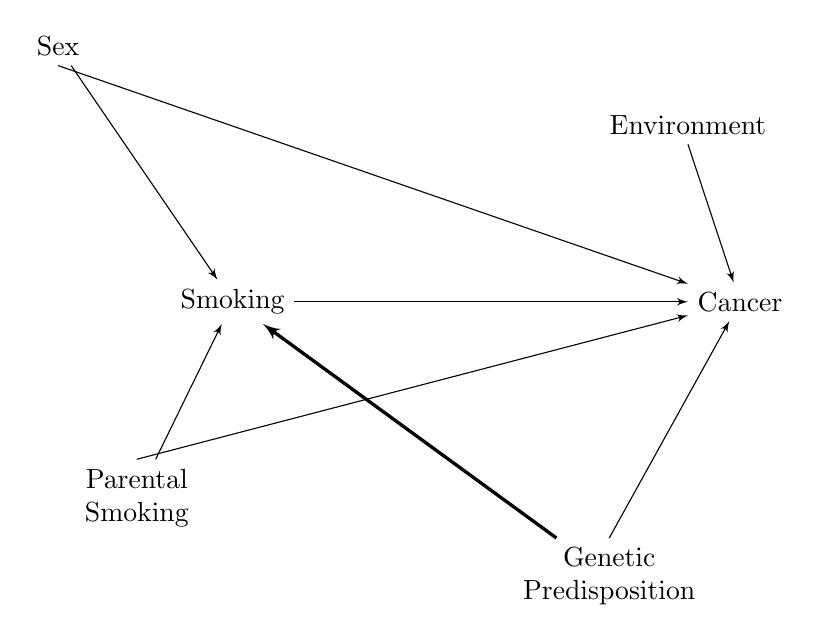
\begin{tikzpicture}[>=latex',circ/.style={draw, shape=circle, node distance=5cm, line width=1.5pt}]
    \draw (0,0) node[left] (X) {Smoking};
    \draw[->] (X) -- (5,0) node[right] (Y) {Cancer};
    \draw<2->[->] (-3,3) node[above] (Z) {Sex} -- (Y);
    \draw<2->[->] (5,2) node[above] (A) {Environment} -- (Y);
    \draw<2->[->] (4,-3) node[below, text width=3cm, align=center] (E) {Genetic\\Predisposition} -- (Y);
    \draw<2->[->] (-2, -2) node[below, text width=2.5cm, align=center] (W) {Parental\\Smoking} -- (Y);
    \draw<3->[->] (Z) -- (X);
    \draw<3->[->] (W) -- (X);
    \draw<4->[->, very thick] (E) -- (X);
\end{tikzpicture}
\end{center}
\end{frame}



\begin{frame}

\frametitle{{\large Causal Graphs I}}

\small

\begin{itemize}\itemsep0.5em
\item Visual representation of (possible) causal relationships
	\begin{itemize}
	\item Called ``directed, acyclic graph'' (DAG)
	\end{itemize}
\item<2-> Causality flows between variables, which are represented as ``nodes''
\item<3-> Variables are causally linked by arrows
\item<4-> Causality only flows \textit{forward}
\item<5-> Nodes creating a ``backdoor path'' from $X$ to $Y$ are confounds
\end{itemize}

\end{frame}


\againframe<3>{smoking-graph}


\frame<1-2>[label=causality]{

\frametitle{{\large 4 (or 5) principles of causality}}

\begin{enumerate}\itemsep1em
\item<2-> Correlation
\item<3-> Nonconfounding
\item<4-> Direction (``temporal precedence'')
\item<5-> Mechanism
\item<6-> (Appropriate level of analysis)
\end{enumerate}
}

\againframe<3>{smoking-graph}

\againframe<3-4>{causality}

\againframe<3-4>{smoking-graph}

\againframe<4-5>{causality}

\againframe<3>{smoking-graph}

\againframe<5-6>{causality}

\frame{
	\centering
	\includegraphics[width=.9\textwidth]{images/brexit-vote-by-age.png}
	
	{\tiny Source: \textit{The Telegraph}. 27 June 2016. \url{http://www.telegraph.co.uk/news/2016/06/24/eu-referendum-how-the-results-compare-to-the-uks-educated-old-an/}\par }
}


\frame{\huge\vskip20pt\textbf{Questions?}}



\section[Counterfactuals]{Fundamental Problem of Causal Inference}
\frame{\tableofcontents[currentsection]}


\frame[label=counterfactuals]{
\frametitle{Counterfactual Thinking}

\begin{itemize}\itemsep1.5em
\item Causal inference involves inferring \textit{what would have happened} in a counterfactual reality \textit{where the potential cause took on a different value}
\item \textit{Counterfactual}: relating to what has not happened or is not the case
\end{itemize}

}

% Has anyone read or seen *A Christmas Carol*?

\frame{
\frametitle{``A Christmas Carol''}

\small 
\begin{itemize}
\item 1843 novel by Charles Dickens
\item Ebenezer Scrooge is shown his own future by the ``Ghost of Christmas Yet to Come''
\item Has the choice to either:
	\begin{itemize}
	\item stay on current path (one counterfactual), or 
	\item change his ways (take a different counterfactual)
	\end{itemize}
\end{itemize}
}

\frame{
\frametitle{{\large Dickensian Causal Inference}}

\begin{itemize}\itemsep1em
\item \textit{Causal effect}: The difference between two ``potential outcomes''
	\begin{itemize}
	\item The outcome that occurs if $X = x_1$
	\item The outcome that occurs if $X = x_2$
	\end{itemize}
\item The causal effect of Scrooge's lifestyle is seen in the \textit{difference(s)} between two potential futures
\end{itemize}

}

\frame{
\frametitle{Fundamental problem of causal inference}

\only<2->{\Large We can only observe any given unit in one reality!}

}

\frame{
\frametitle{Two solutions!\footnote{From Holland}}

\begin{enumerate}\itemsep1em
\item Scientific Solution
	\begin{itemize}
	\item All units are identical
	\item Each can provide a perfect counterfactual
	\item Common in, e.g., agriculture, biology
	\end{itemize}
\item<2-> Statistical Solution
	\begin{itemize}
	\item Units are not identical
	\item Random exposure to a potential cause
	\item Effects measured on average across units
	\item Known as the ``Experimental ideal''
	\end{itemize}
\end{enumerate}

}


\frame<1>[label=mill]{

\frametitle{Mill's methods\footnote{Discussed in Holland}}

\begin{itemize}
\item Agreement
\item \textbf<2>{Difference}
\item Agreement and Difference
\item Residue
\item Concomitant variations
\end{itemize}
}

\frame{
\frametitle{{\normalsize Mill's Method of Difference}}

If an instance in which the phenomenon under investigation occurs, and an instance in which it does not occur, have every circumstance save one in common, that one occurring only in the former; the circumstance in which alone the two instances differ, is the effect, or cause, or an necessary part of the cause, of the phenomenon.
}


\frame{

\frametitle{{\large ``Rerum cognoscere causas''}}

\begin{itemize}
\item<1-> Causal inference is meant to help ``explain'' the world
	\begin{itemize}
	\item<2-> Other notions of explain (e.g., description)
	\item<3-> Explanation may or may not involve mechanistic claims (see LT Week 5)
	\end{itemize}
\item<4-> Causation is deterministic at the unit level!
\item<5-> Counterfactual approaches to causal inference are ``forward'' in nature
\end{itemize}

}

\frame{
\centering
Prediction is not causation.\\ Causation is not prediction.

\vspace{2em}

\only<2->{Why are these distinct?}

}




\section{Randomized Experiments}
\frame{\tableofcontents[currentsection]}





% Individual-level effects versus ATEs


\frame{
	\frametitle{The Experimental Ideal}
	\small
	A randomized experiment, or randomized control trial is:
 		\begin{quote}\small
 			The observation of units after, and possibly before, a randomly assigned intervention in a controlled setting, which tests one or more precise causal expectations
 		\end{quote}
 	This is Holland's ``statistical solution'' to the fundamental problem of causal inference
}

\frame{
	\frametitle{Random Assignment}

\small
\begin{itemize}\itemsep0.5em
\item A physical process of randomization
	\begin{itemize}\small
	\item Breaks the ``selection process''
	\item Units only take value of $X = x$ because of assignment
	\end{itemize}
\item<2-> This means:
	\begin{itemize}\small
	\item Treatment groups, on average, provide in sight into counterfactual ``potential'' outcomes
	\item Randomization means potential outcomes are balanced between groups, so no confounding
	\end{itemize}
\end{itemize}

}

\begin{frame}
\small 
\begin{center}
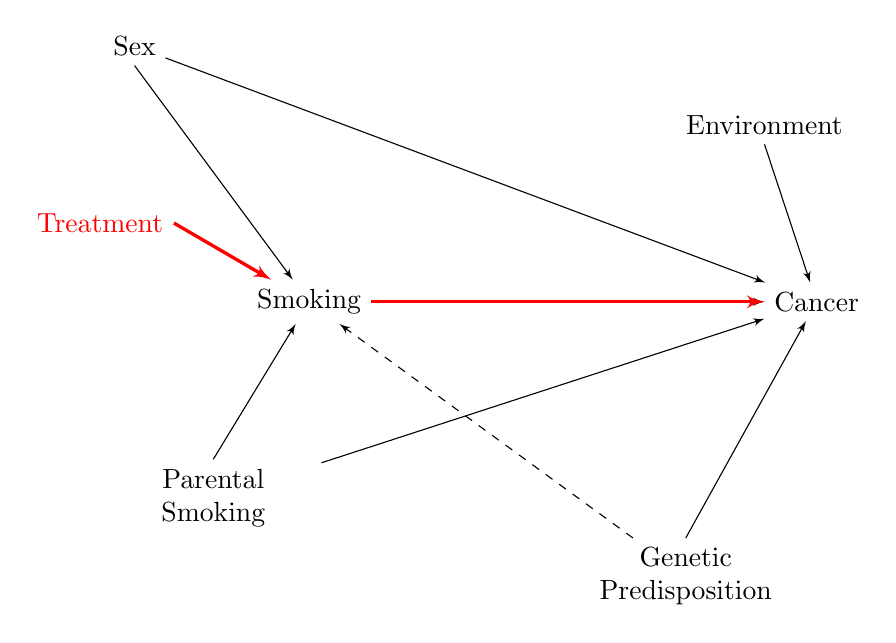
\begin{tikzpicture}[>=latex',circ/.style={draw, shape=circle, node distance=5cm, line width=1.5pt}]
    \draw[->] (0,0) node[left] (X) {Smoking} -- (5,0) node[right] (Y) {Cancer};
    \draw[->] (-3,3) node[above] (Z) {Sex} -- (X);
    \draw[->] (Z) -- (Y);
    \draw[->] (5,2) node[above] (A) {Environment} -- (Y);
    \draw[->] (4,-3) node[below, text width=3cm, align=center] (E) {Genetic\\Predisposition} -- (Y);
    \draw[->] (-2, -2) node[below, text width=2.5cm, align=center] (W) {Parental\\Smoking} -- (X);
    \draw[->] (W) -- (Y);
    \draw[->, dashed] (E) -- (X);
    
    \draw<2->[->, very thick, color=red] (-2.5,1) node[left, color=red] (Tr) {Treatment} -- (X);
    \draw<2->[->, very thick, color=red] (X) -- (Y);
\end{tikzpicture}
\end{center}
\end{frame}



% design-based experimental inference
\frame{
	\frametitle{Experimental Inference I}
	\small
	\begin{itemize}\itemsep0.5em
    	\item<1-> Causal inference is a comparison of two \textit{potential outcomes}
    	\item<2-> A potential outcome is the value of the outcome (Y) for a given unit (i) after receiving a particular version of the treatment (X)
    	\item<3-> Each unit has multiple \textit{potential} outcomes ($Y_{0i}$, $Y_{1i}$), but we only observe one of them
    	\item<4-> A \textit{causal effect} is the difference between these (e.g., $Y_{X=1} - Y_{X=0}$), all else constant
	\end{itemize}
}

\frame{
	\frametitle{Experimental Inference II}
	\small
	\begin{itemize}\itemsep0.5em
    	\item<1-> We cannot see individual-level causal effects
			\begin{itemize}
			\item<1-> We want to know: $TE_i = Y_{1i} - Y_{0i}$
			\end{itemize}
    	\item<2-> We can see \textit{average causal effects}
    		\begin{itemize}
        		\item<2-> Ex.: Average difference in cancer between those who do and do not smoke
        		\item<2-> $ATE_{naive} = E[Y_{1i} | X = 1] - E[Y_{0i} | X = 0]$
    		\end{itemize}
    	\item<3-> Is this what we want to know?
    		\begin{itemize}
    		\item<4-> Yes, if $X$ randomized
    		\item<5-> Yes, if all confounds controlled
    		\end{itemize}
	\end{itemize}
}


\frame{}




\frame{

\frametitle{Preview of next week}

\begin{itemize}\itemsep1em
\item What is a ``scientific literature''?
\item How do we accumulate scientific evidence?
\end{itemize}

}


\appendix
\frame{}

\frame{\frametitle{Mill's Methods}}

\frame{
\frametitle{Agreement}

If two or more instances of the phenomenon under investigation have only one circumstance in common, the circumstance in which alone all the instances agree, is the cause (or effect) of the given phenomenon.
}

\frame{
\frametitle{Difference}

If an instance in which the phenomenon under investigation occurs, and an instance in which it does not occur, have every circumstance save one in common, that one occurring only in the former; the circumstance in which alone the two instances differ, is the effect, or cause, or an necessary part of the cause, of the phenomenon.
}

\frame{
\frametitle{Agreement and Difference}

If two or more instances in which the phenomenon occurs have only one circumstance in common, while two or more instances in which it does not occur have nothing in common save the absence of that circumstance; the circumstance in which alone the two sets of instances differ, is the effect, or cause, or a necessary part of the cause, of the phenomenon.
}

\frame{
\frametitle{Residue}

Subduct from any phenomenon such part as is known by previous inductions to be the effect of certain antecedents, and the residue of the phenomenon is the effect of the remaining antecedents.
}

\frame{
\frametitle{Concomitant variations}

Whatever phenomenon varies in any manner whenever another phenomenon varies in some particular manner, is either a cause or an effect of that phenomenon, or is connected with it through some fact of causation.
}


\end{document}
